\documentclass{beamer}
%\documentclass[handout,xcolor=pdftex,dvipsnames,table]{beamer}

%\usetheme{AP}


\usepackage[dutch]{babel}
\usepackage{pdfpages}

\title[]{ARM Architectuur}
\subtitle{}
\author{}
\institute{Jeroen Doggen \\ jeroen.doggen@ap.be}
\date{Versie: \today}

\begin{document}

% Titlepage 
\maketitle

% Outline Page
\section*{Overzicht}
\begin{frame}
\frametitle{Overzicht}
\tableofcontents[pausesections]
\end{frame}


\section{ARM Overzicht}
% Outline Page
\begin{frame}
\frametitle{Overzicht}
\tableofcontents[sectionstyle=show/shaded,subsectionstyle=show/shaded] 
\end{frame}

\begin{frame} 
\frametitle{ARM Overzicht}
\begin{figure}[h] \begin{center}
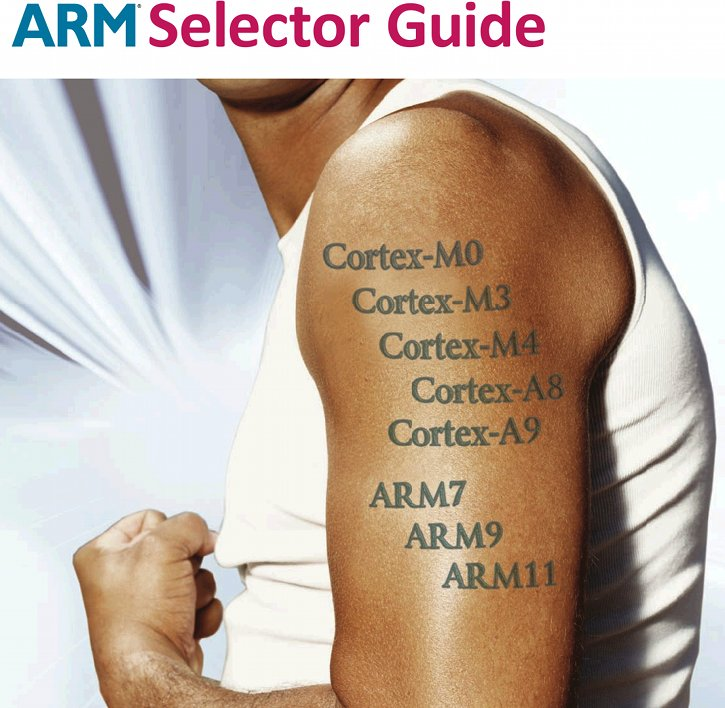
\includegraphics[width=0.67\textwidth]{figures/armarm.jpeg}
\end{center} \end{figure}
\end{frame}

\begin{frame} 
\frametitle{ARM Overzicht}

\begin{itemize}
 \item <1-> Opgericht in november 1990, spin-off van Acorn Computers \footnote{http://en.wikipedia.org/wiki/Acorn\_Computers}
 \item <2-> ARM verkoopt licenties van de ARM core aan halfgeleider partners die ARM chips fabriceren en verkopen aan hun klanten
  \begin{itemize}
    \item ARM fabriceert zelf geen chips
    \end{itemize}
 \item <3-> ARM is de grootste speler op het gebied van 32-bit embedded microprocessoren.
 \item <4-> ARM biedt een breed scale aan architecturen en modellen aan:
      \begin{itemize}
	\item Hoge performance, lage kostprijs, laag energieverbruik
      \end{itemize}
 \item <5-> ARM biedt samen met zijn partners teven tools en software aan die ontwikkeling van embedded applicaties zo makkelijk en effici\"ent mogelijk te maken.
 \item <6-> Er werden reeds 20 miljard processoren gemaakt en momenteel worden meer dan 10 miljoen processoren per dag afgeleverd. 
\end{itemize}
\begin{figure}[h] \begin{center}

\includegraphics[width=0.13\textwidth]{figures/armlogo.jpg}
\end{center} \end{figure}
\end{frame}

\begin{frame} 
\frametitle{ARM Partnership model}
\begin{figure}[h] \begin{center}
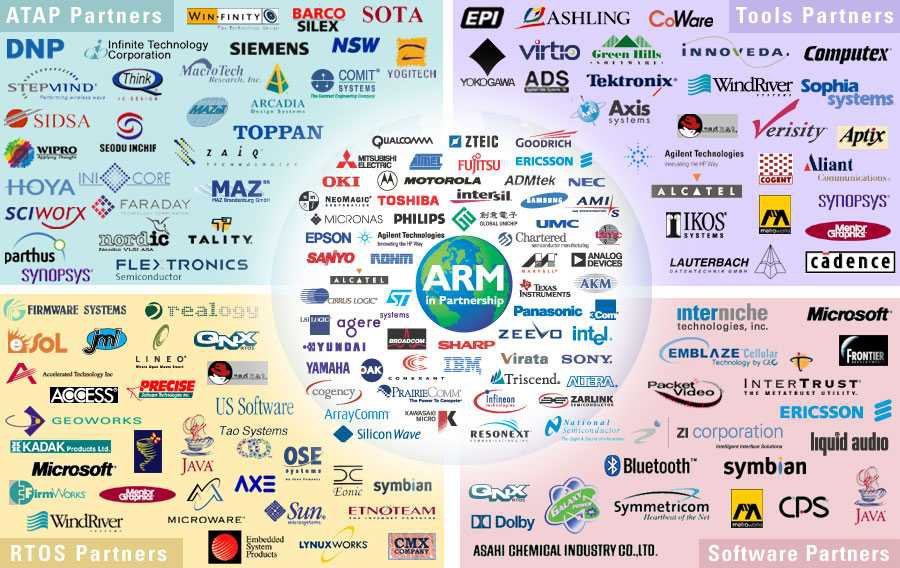
\includegraphics[width=0.99\textwidth]{figures/armpartners.jpeg}
\end{center} \end{figure}
\end{frame}

\begin{frame} 
\frametitle{Elektronica met ARM core}
\begin{figure}[h] \begin{center}
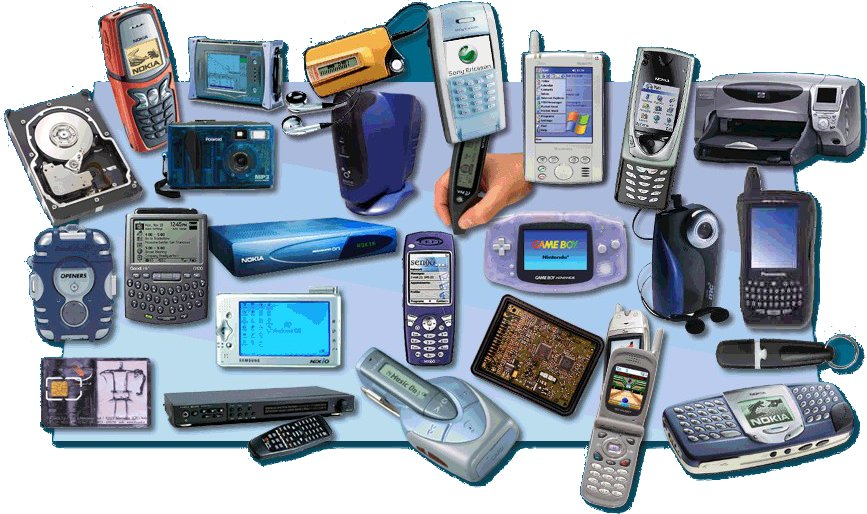
\includegraphics[width=0.99\textwidth]{figures/armdevices.jpeg}
\end{center} \end{figure}
\end{frame}

\begin{frame} 
\frametitle{Intellectueel eigendom}
  \begin{itemize}
    \item <1-> De verschillende ARM cores delen een gemeenschappelijke instructieset.   
    \item <2-> ARM biedt de volledige interne werking aan halfgeleider partners aan.
	\begin{itemize}
	\item Hard en soft views (gate level netlist).
	\end{itemize}
    \item <3-> OEMS krijgen enkel beschikking over de hard view. (ter bescherming van IP).
  \end{itemize}

\end{frame}

\section{ARM Programmeermodel}
% Outline Page
\begin{frame}
\frametitle{Overzicht}
\tableofcontents[sectionstyle=show/shaded,subsectionstyle=show/shaded] 
\end{frame}

\begin{frame} 
\frametitle{ARM Programmeermodel}
\begin{itemize}
 \item <1-> ARM is een 32-bit architectuur.
 \item <2-> Wanneer deze termen worden gebruikt in de ARM context:
    \begin{itemize}
    \item Byte: 8 bits
    \item Halfword: 16 bits
    \item Word: 32 bits
    \end{itemize}
 \item <3-> De meeste ARM's implementeren twee instructiesets:
    \begin{itemize}
    \item 32-bit ARM instructieset
    \item 16-bit Thumb instructieset
    \end{itemize}
 \item <4-> Jazelle cores kunnen ook Java bytecode uitvoeren. (native)
\end{itemize}
\end{frame}

\subsection{Classic ARM processors}
% Outline Page
\begin{frame}
\frametitle{Overzicht}
\tableofcontents[sectionstyle=show/shaded,subsectionstyle=show/shaded] 
\end{frame}

\begin{frame} 
\frametitle{ARM 1 tot 6}
\begin{itemize}
 \item <1-> ARMv1 tot ARMv3 architectuur.
 \item <2-> Tussen 1985 en +/- 1995 werden vele modellen van ARM processoren ontwikkeld.
 \item <3-> De meeste van deze processoren worden nu niet vaak meer gebruikt in nieuwe producten.
\end{itemize}
\begin{figure}[h] \begin{center}
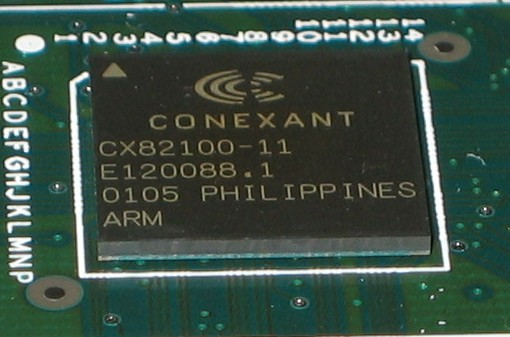
\includegraphics[width=0.4\textwidth]{figures/conexant-arm.jpg}
\caption{Een Conexant ARM processor, voornamelijk gebruikt in routers}rtesis
\end{center} \end{figure}
\end{frame}

\begin{frame} 
\frametitle{ARM 7}
\begin{itemize}
 \item <1-> De meest gebruikte ARM7 designs implementeren de ARMv4T architectuur. (Von Neumann)
 \item <2-> Deze generatie introduceerde de Thumb 16-bit instructieset: verbeterde code densiteit t.o.v. voorgaande designs.
 \item <3-> E\'en historisch belangrijk model is de ``ARM7DI'': deze introduceerde JTAG debugging. \footnote{http://www.jtag.com/en/Learn/Standards/IEEE\_1149.1}
      \begin{itemize}
      \item JTAG wordt veel gebruikt voor het testen van PCB's
      \item Biedt de mogelijkheid om stap per stap code uit te laten voeren: single stepping \& breakpointing
      \end{itemize}
 \item <4-> Bekende elektronica waarin deze chip gebruikt wordt:
      \begin{itemize}
      \item iPod, Nintendo DS, Game Boy Advance, routers,...
      \end{itemize}
\end{itemize}
\end{frame}

\begin{frame} 
\frametitle{Digital Signal Processing (DSP)}
\begin{itemize}
 \item <1-> Een analoog signaal wordt gesampled en gekwantiseerd
 \item <2-> Het digitaal wordt digitaal bewerkt (filter, echo, ...)
    \begin{itemize}
     \item <3-> MAC instructie: \textbf{M}ultiply, \textbf{A}dd \& \textbf{A}ccumulate \footnote{Meer info: cursus embedded systems 5}
    \end{itemize}
 \item <4-> Het bewerkt signaal wordt terug in analoge vorm omgezet
\end{itemize}rtesis
\begin{figure}[h] \begin{center}
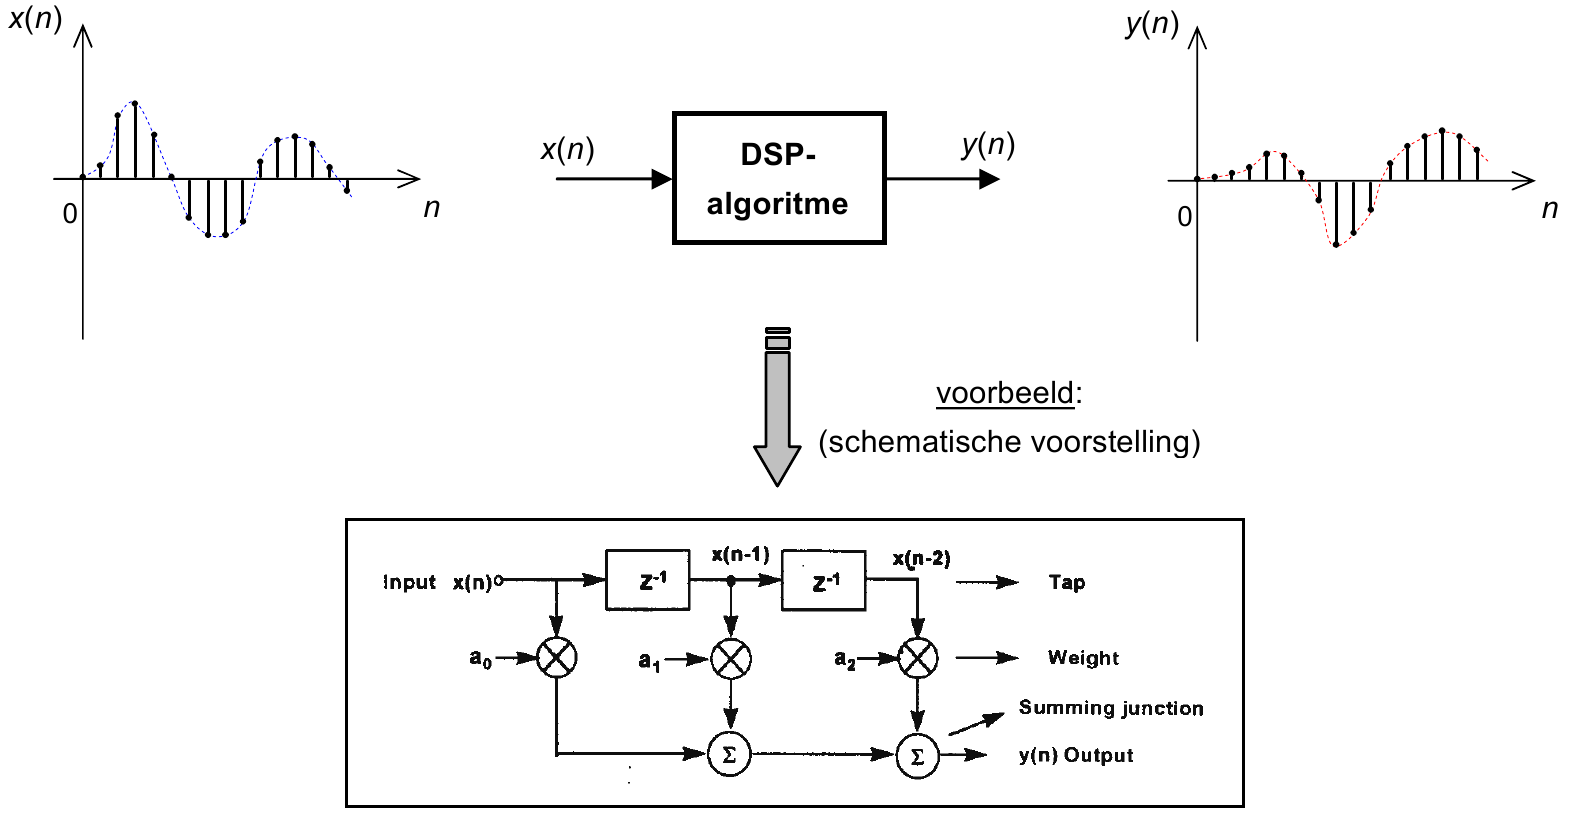
\includegraphics[width=0.8\textwidth]{figures/dsp.png}
\end{center} \end{figure}
\end{frame}

\begin{frame} 
\frametitle{ARM 9}
  \begin{itemize}
  \item <1-> ARM9 is een 32-bit RISC architectuur. (ARMv4T en ARMv5TE)
  \item <2-> Bij deze generatie verandere ARM van de Von Neuman naar de Harvard architectuur met een aparte data en instructiebus waardoor de snelheid significant kan toenemen.
  \item <3-> Verbeteringen t.o.v. ARM7
      \begin{itemize}
      \item <4-> Lagere warmteproductie en minder risico op oververhitting.
      \item <5-> Hogere kloksnelheden en langere pipeline.
      \item <6-> Klokcycli verbeteringen: vele instructies worden nu in \'e\'en cyclus voltooid.
      \item <7-> Sommige ARM9 cores beschikken over ``Enhanced DSP'' instructies (bijv. MAC) voor digitale signaalverwerking algoritmes.
      \end{itemize}
  \item <8-> Bekende elektronica waarin deze chip gebruikt wordt:
      \begin{itemize}
      \item Nintendo DSi, eReaders, NAS, routers, GSM's ...
      \end{itemize}
  \end{itemize}
\end{frame}

\begin{frame} 
\frametitle{ARM 11}
  \begin{itemize}
  \item <1-> De ARM11 introduceerde de ARMv6 architectuur.
  \item <2-> Verbeteringen t.o.v. ARM9
	\begin{itemize}
	\item <3-> SIMD instructies voor betere multimedia toepassingen.
	\item <4-> Lagere warmteproductie en minder risico op oververhitting.
	\item <5-> Hogere kloksnelheden en langere pipeline.
	\item <6-> Sommige ARM9 cores beschikken over ``Enhanced DSP'' instructies (bijv. MAC) voor digitale signaalverwerking algoritmes.
	\end{itemize}
  \item <7-> Bekende elektronica waarin deze chip gebruikt wordt:
	\begin{itemize}
	\item HTC, Nokia, Samsung smartphones, Apple iPhone, iPod Touch, Amazon Kindle,...
	\end{itemize}
  \end{itemize}
\end{frame}


\subsection{Embedded ARM processors}
% Outline Page
\begin{frame}
\frametitle{Overzicht}
\tableofcontents[sectionstyle=show/shaded,subsectionstyle=show/shaded] 
\end{frame}

\begin{frame} 
\frametitle{ARM Cortex-M0}
  \begin{itemize}
  \item <1-> De ARM Cortex-M0 processor is de kleinste, meest energie zuinige ARM processor.
  \item <2-> Door het zeer kleine silicon oppervlak en minimale code footpint levert deze processor 32-bit performance bij een 8-bit verkoopsprijs.
  \item <3-> Key features: (NXP LPC1100 Series)
	\begin{itemize}
	\item 50 MHz, 32-bit, tto 32 kB Flash, 8 kB SRAM
	\item UART, SPI, $I^2C$,  8-channel 10 bit AD-converter, 42 GPIO
	\item Active power: $150\mu A / MHz$
	\item Drie laag vermogen standen: sleep, deep-sleep en deep power-down
	\item Wakup door timer, interrupt
	\item Pin to pin compatible met LPC1300 (Cortex M3)
	\end{itemize}
  \end{itemize}
\end{frame}

\begin{frame} 
\frametitle{ARM Cortex-M1}
  \begin{itemize}
  \item <1-> De ARM Cortex-M1 processor is specifiek gericht op FPGA implementaties.
  \item <2-> De key features zijn vergelijkbaar met de Cortex-M0
  \end{itemize}
\begin{figure}[h] \begin{center}
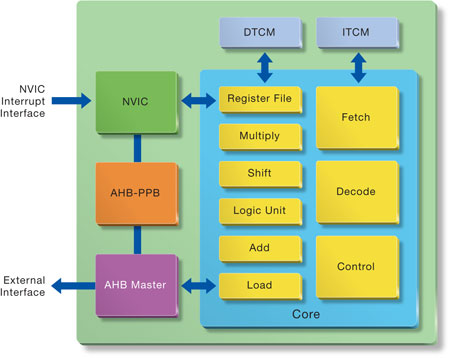
\includegraphics[width=0.6\textwidth]{figures/armM1.png}
\end{center} \end{figure}
\end{frame}

\begin{frame} 
\frametitle{ARM Cortex Mx}
\begin{figure}[h] \begin{center}
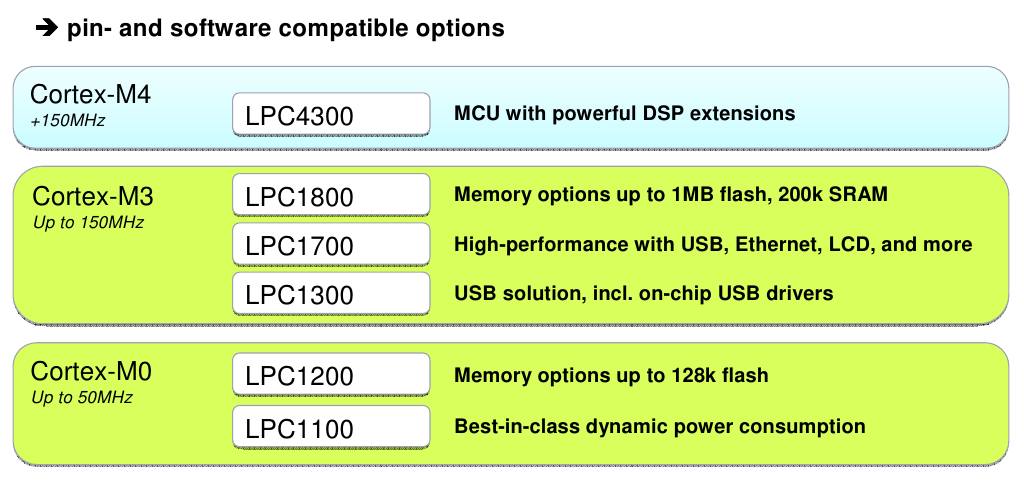
\includegraphics[width=0.99\textwidth]{figures/arm-cortex.png}
\end{center} \end{figure}
\end{frame}

\begin{frame} 
\frametitle{ARM Cortex Mx}
\begin{figure}[h] \begin{center}
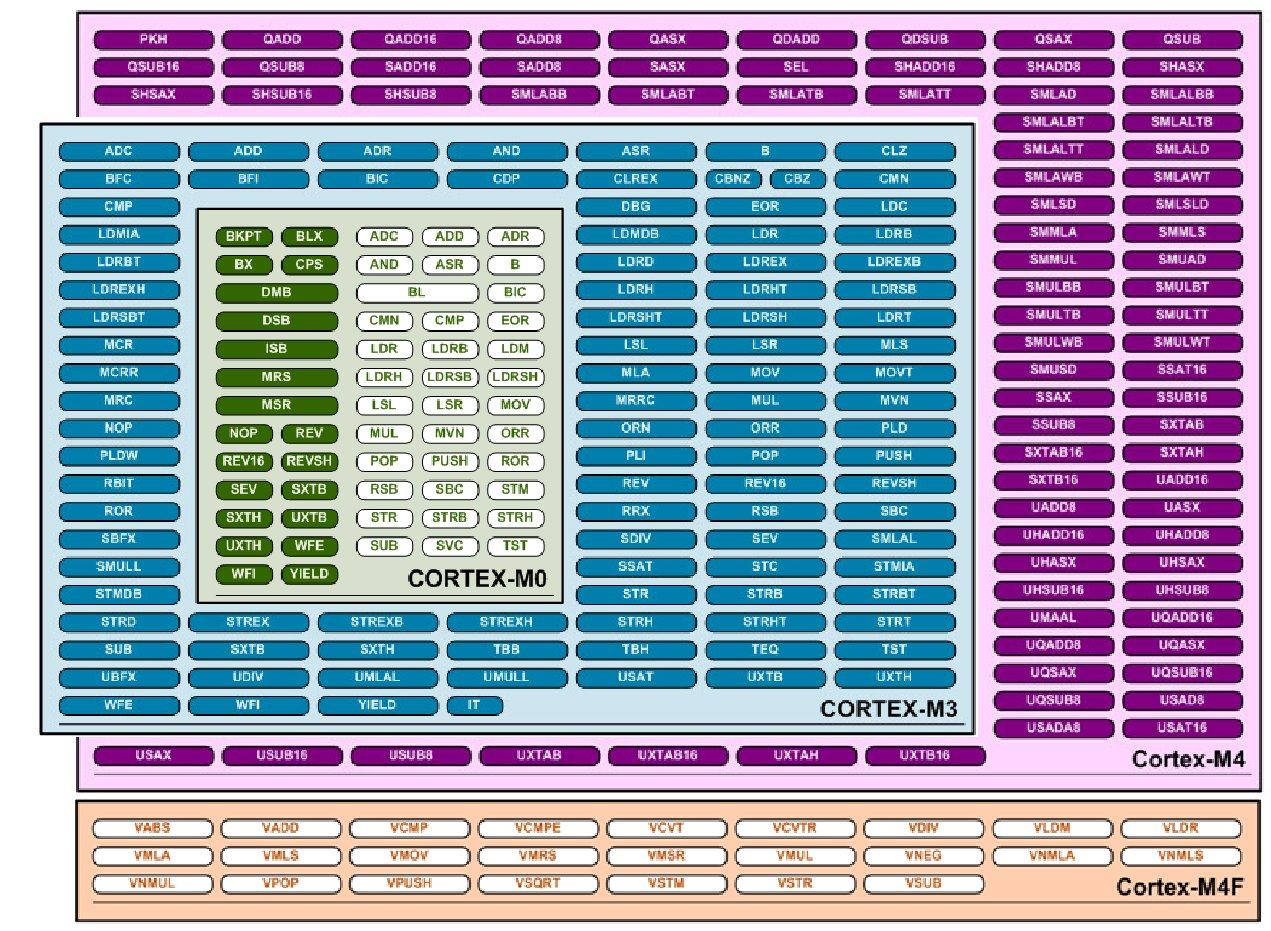
\includegraphics[width=0.9\textwidth]{figures/arm-instr.jpeg}
\end{center} \end{figure}
\end{frame}

\begin{frame} rtesis
\frametitle{ARM Cortex Mx}
\begin{figure}[h] \begin{center}
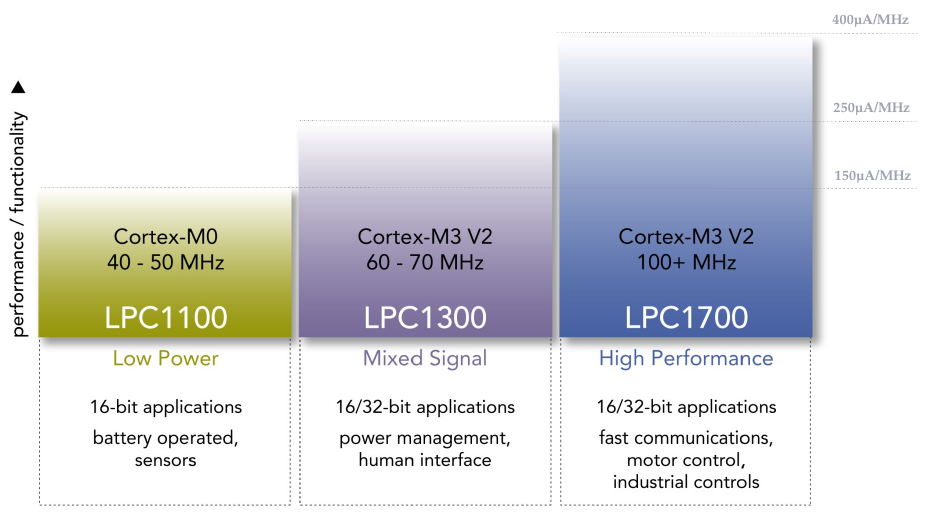
\includegraphics[width=0.99\textwidth]{figures/arm-cortex2.png}
\end{center} \end{figure}
\end{frame}

\begin{frame} 
\frametitle{ARM Cortex Mx}
\begin{figure}[h] \begin{center}
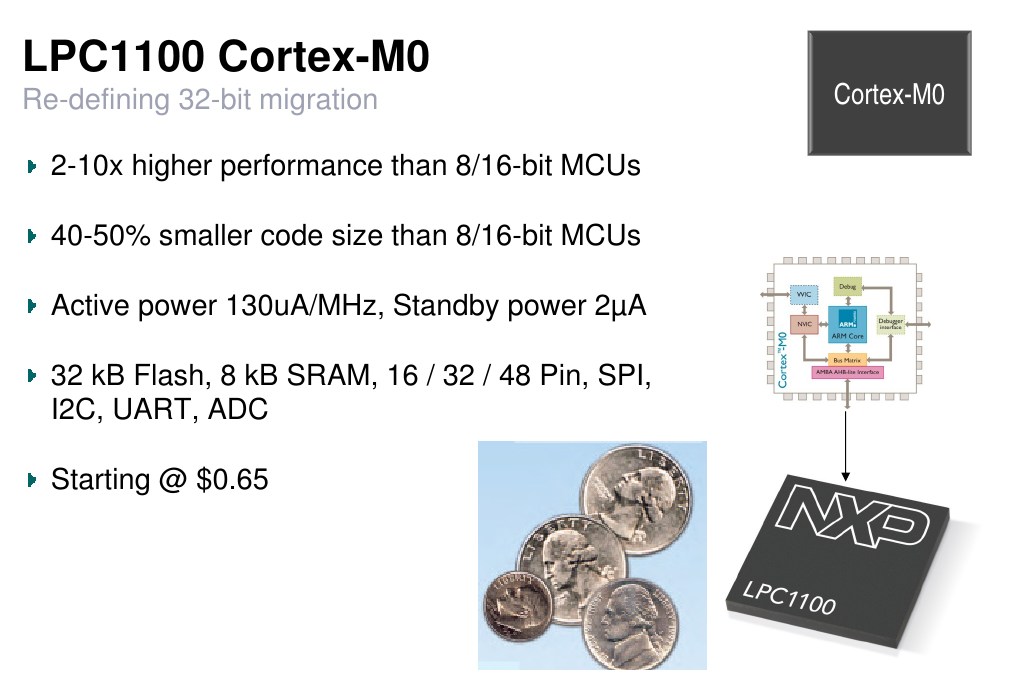
\includegraphics[width=0.99\textwidth]{figures/arm-cortex3.png}
\end{center} \end{figure}
\end{frame}

\begin{frame} 
\frametitle{ARM Cortex Mx}
\begin{figure}[h] \begin{center}
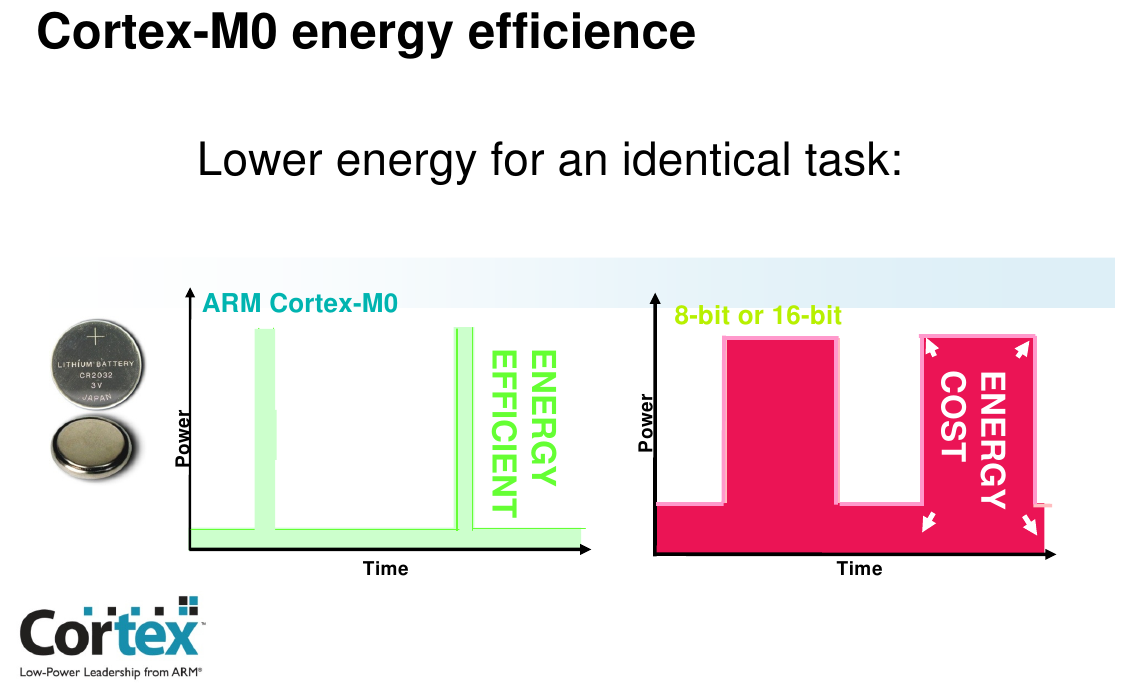
\includegraphics[width=0.99\textwidth]{figures/arm-cortex4.png}
\end{center} \end{figure}
\end{frame}

\begin{frame} 
\frametitle{ARM Cortex Mx}
\begin{figure}[h] \begin{center}
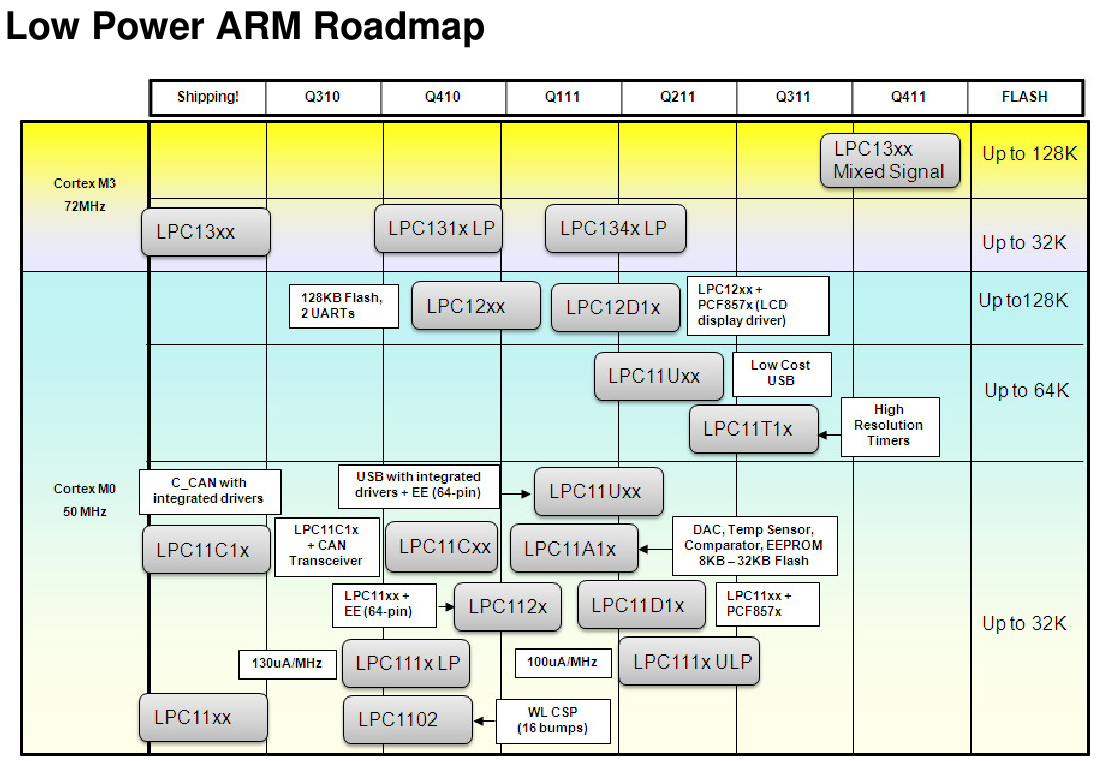
\includegraphics[width=0.9\textwidth]{figures/arm-lowproad.png}
\end{center} \end{figure}
\end{frame}

% \begin{frame} 
% \frametitle{ARM Cortex Mx}
% \begin{figure}[h] \begin{center}rtesis
% 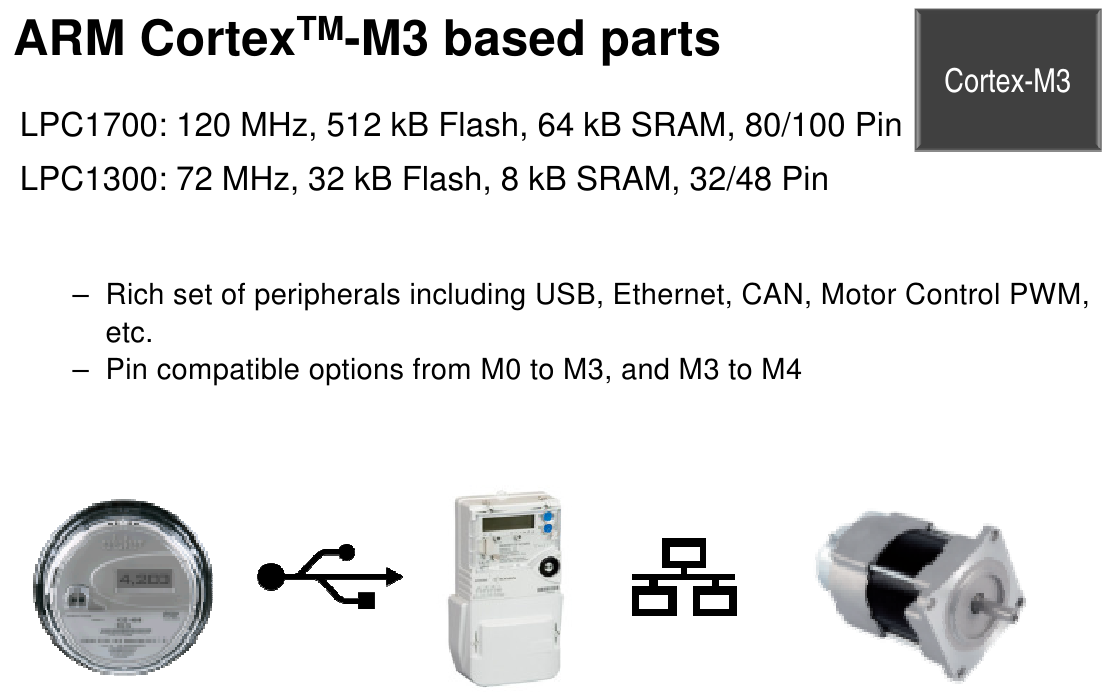
\includegraphics[width=0.99\textwidth]{figures/arm-cortex5.png}
% \end{center} \end{figure}
% \end{frame}
% 
% \begin{frame} 
% \frametitle{ARM Cortex Mx}
% \begin{figure}[h] \begin{center}
% 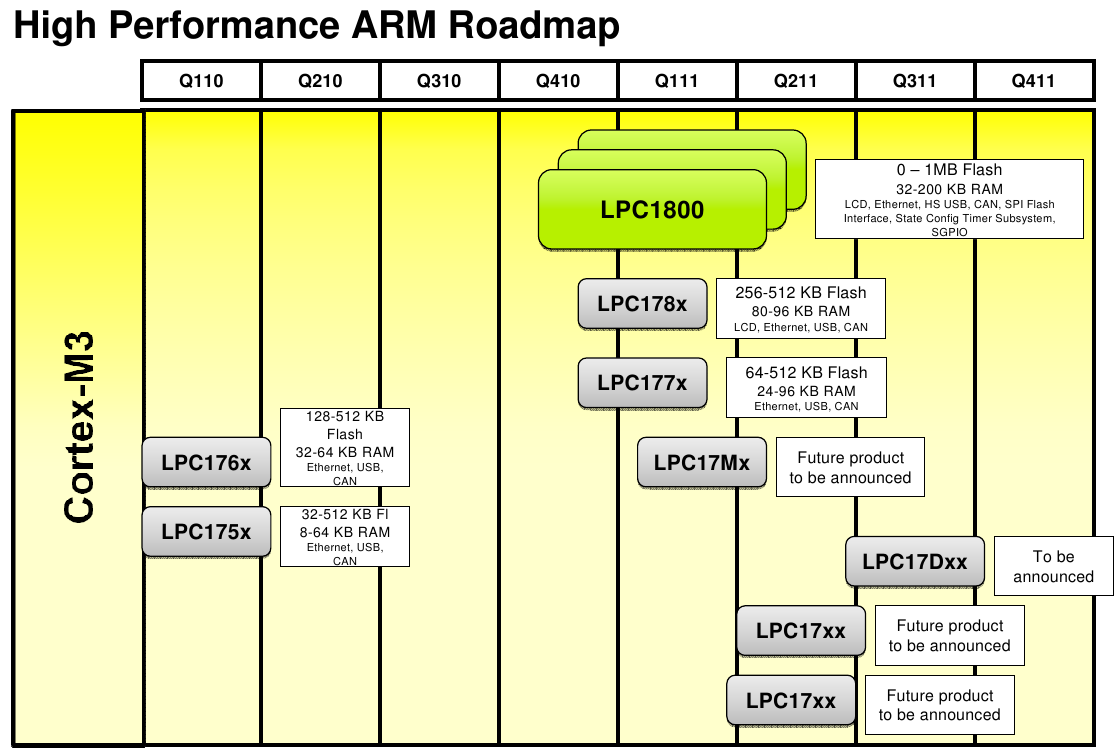
\includegraphics[width=0.99\textwidth]{figures/arm-highproad.png}
% \end{center} \end{figure}
% \end{frame}
% 
% \begin{frame} 
% \frametitle{ARM Cortex Mx}
% \begin{figure}[h] \begin{center}
% 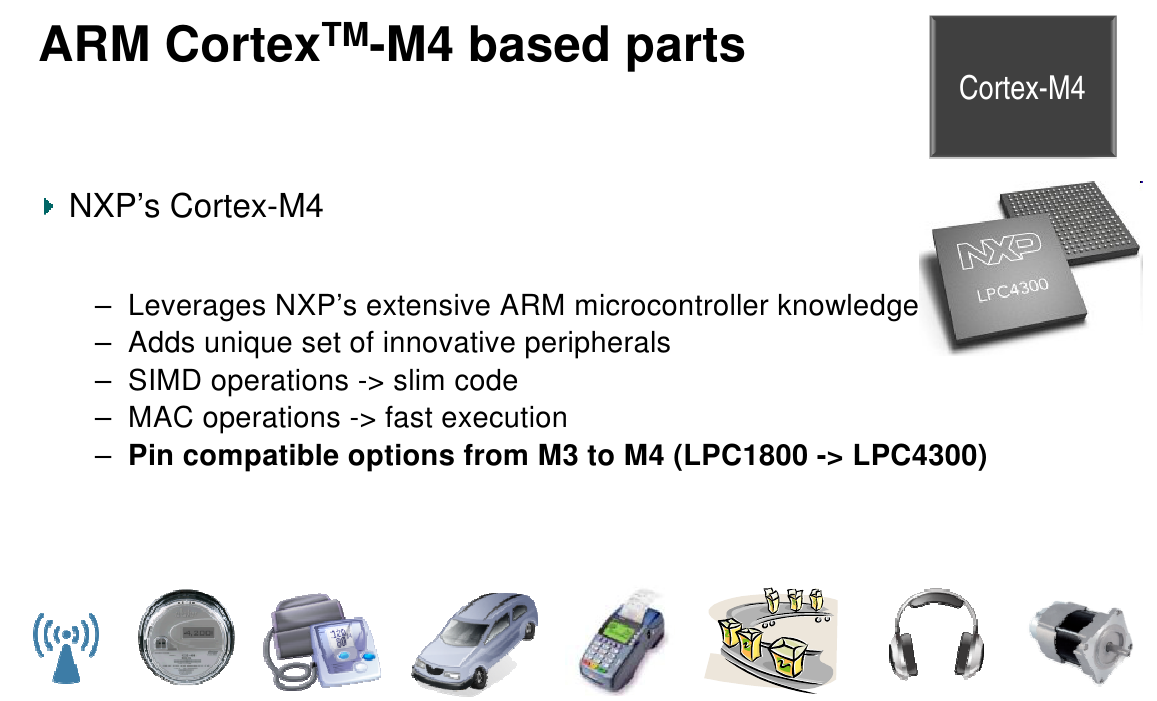
\includegraphics[width=0.99\textwidth]{figures/arm-cortex6.png}
% \end{center} \end{figure}
% \end{frame}
% 
% \begin{frame} 
% \frametitle{ARM Cortex Mx}
% \begin{figure}[h] \begin{center}
% 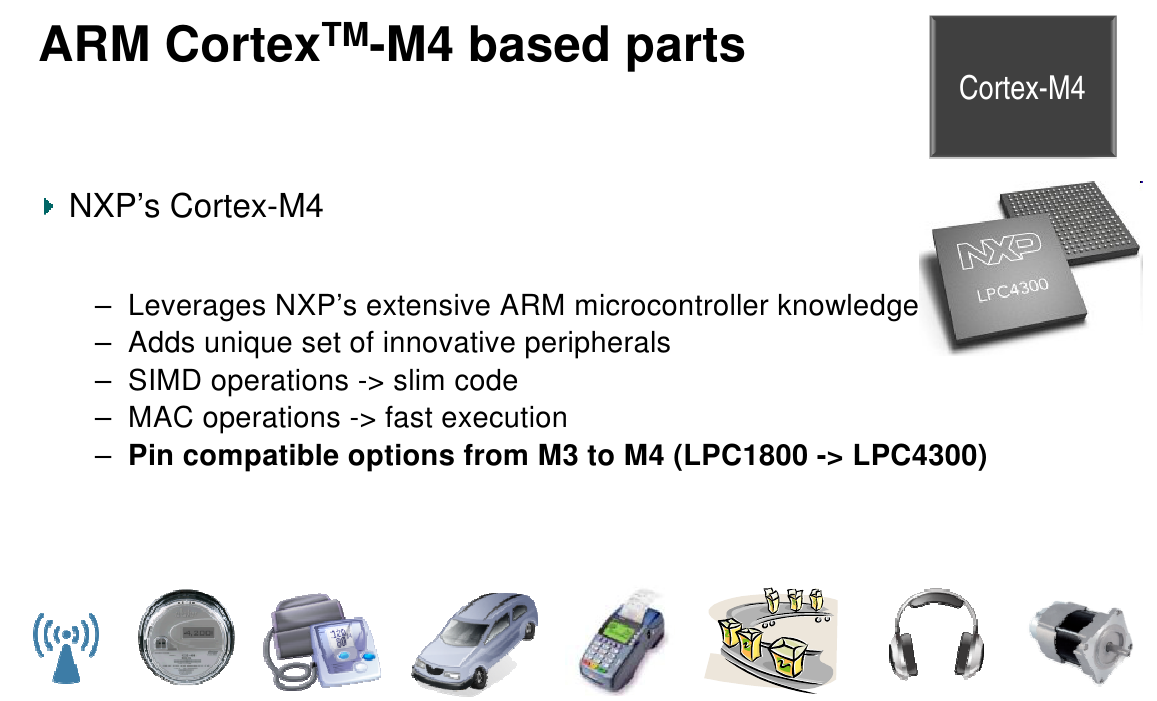
\includegraphics[width=0.99\textwidth]{figures/arm-cortex6.png}
% \end{center} \end{figure}
% \end{frame}
% 
% \begin{frame} 
% \frametitle{ARM Cortex Mx}
% \begin{figure}[h] \begin{center}
% 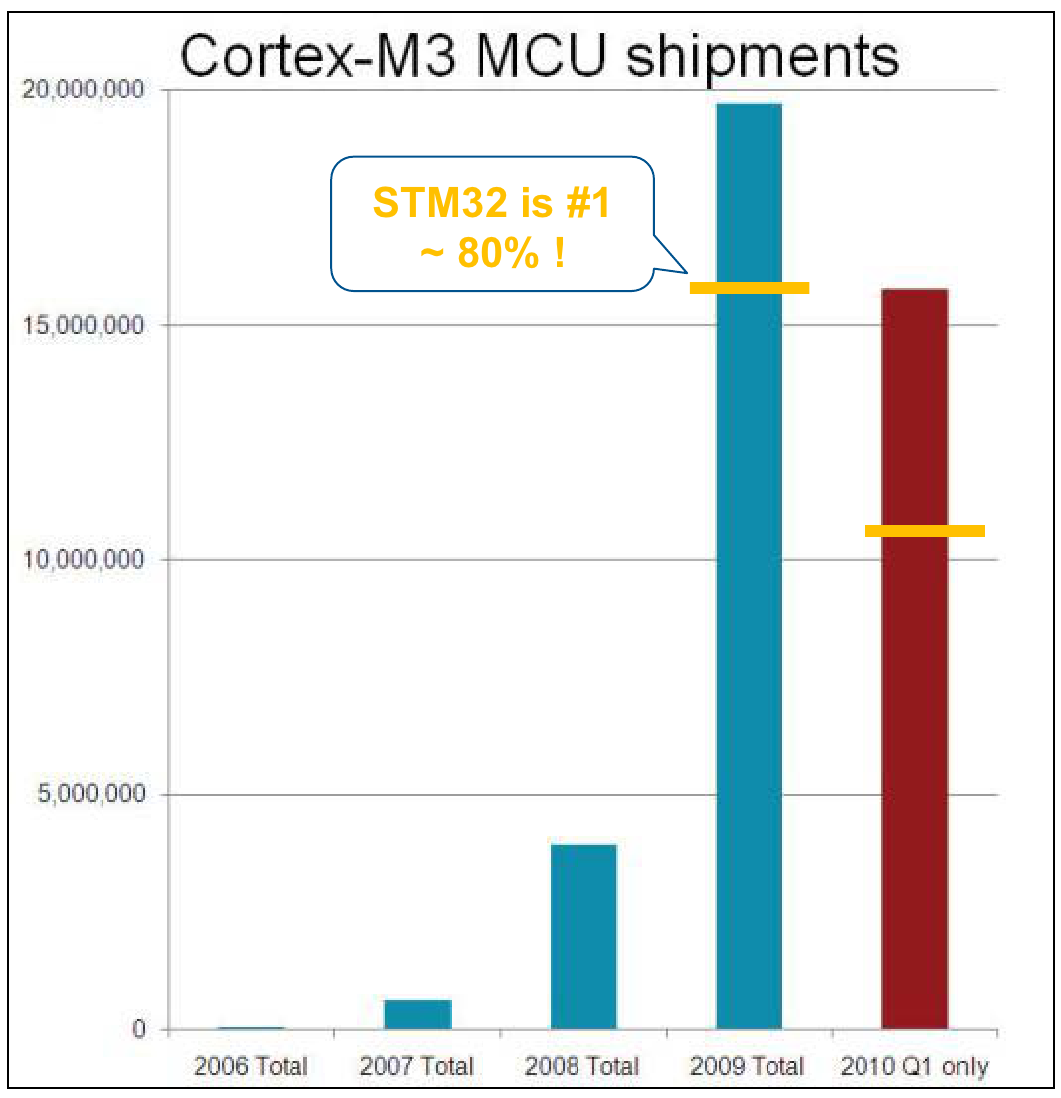
\includegraphics[width=0.64\textwidth]{figures/arm-cortexM3.png}
% \end{center} \end{figure}
% \end{frame}
% 
% \begin{frame} 
% \frametitle{ARM Cortex Mx}
% \begin{figure}[h] \begin{center}
% 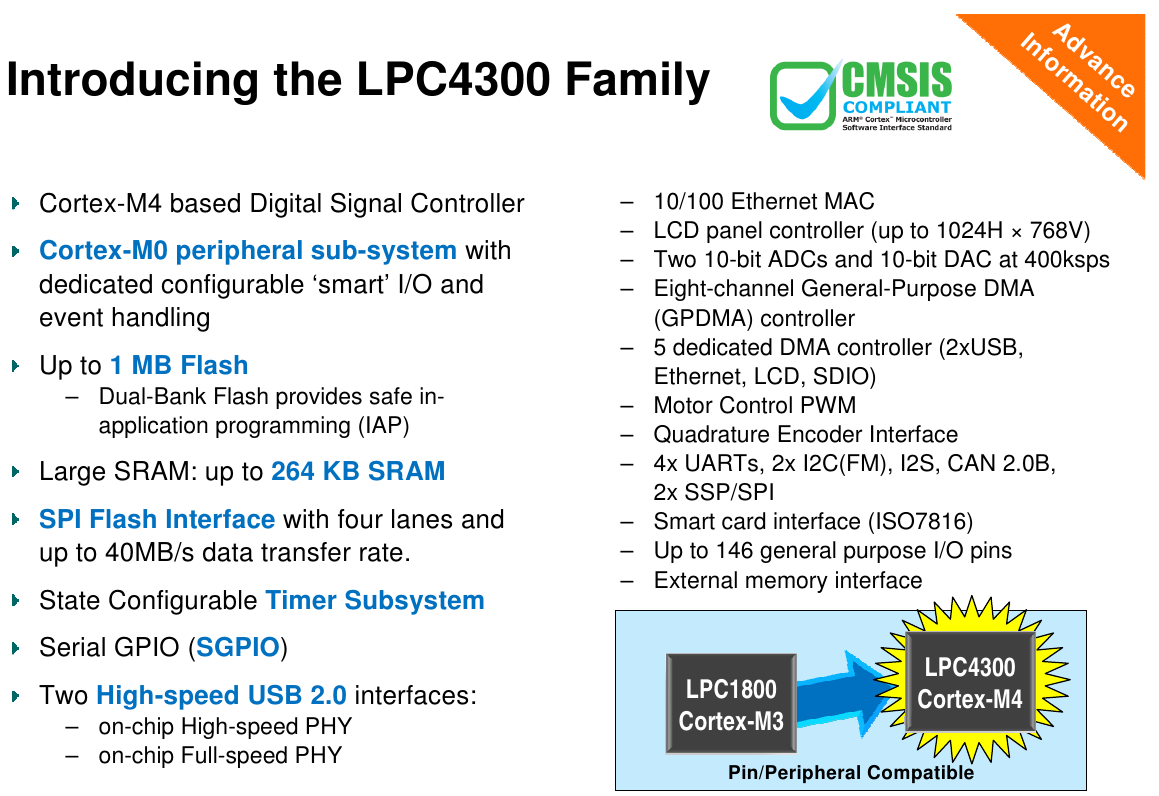
\includegraphics[width=0.9\textwidth]{figures/arm-cortex7.png}
% \end{center} \end{figure}
% \end{frame}
% 
\begin{frame} 
\frametitle{ARM Cortex M3}
%$P=CV^2f$
\begin{figure}[h] \begin{center}
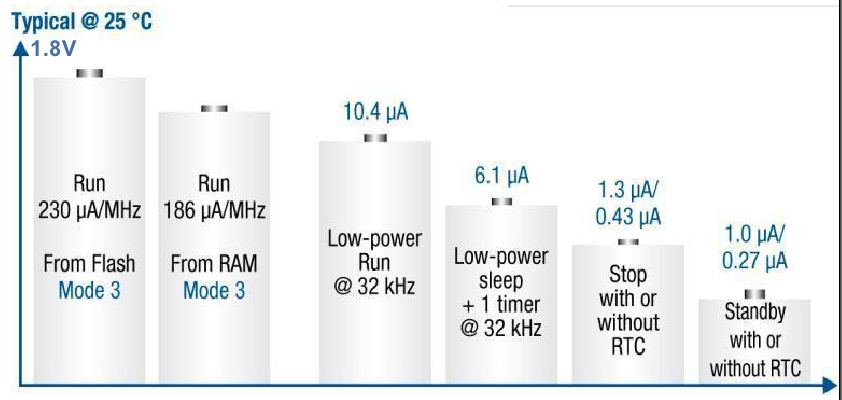
\includegraphics[width=0.99\textwidth]{figures/arm-cortexM3power.png}
\end{center} \end{figure}
\end{frame}

% \begin{frame} 
% \frametitle{ARM Cortex M4}
% \end{frame}
% 
% \begin{frame} 
% \frametitle{ARM Cortex R4}
% \end{frame}


\subsection{Application ARM processors}
% Outline Page
\begin{frame}
\frametitle{Overzicht}
\tableofcontents[sectionstyle=show/shaded,subsectionstyle=show/shaded] 
\end{frame}

\begin{frame} 
\frametitle{ARM Cortex-A8}
    \begin{itemize}
      \item <1-> De ARM Cortex-A8 processor is de huidige mainstream smarthone processor.
      \item <2-> De key features:
      \begin{itemize}
	  \item Frequentie van 600 MHz tot 1.5 GHz.
	  \item Superscalar dual-issue microarchitecture.
	  \item NEON SIMD instruction set extension (optional).
	  \item VFPv3 Floating Point Unit (optional).
	  \item Thumb-2 instruction set encoding.
	  \item Jazelle RCT.
	  \item Advanced branch prediction unit with $>$95 $\%$ accuracy.
	  \item Integrated Level 2 Cache (0-4 MB).
	  \item 2.0 DMIPS / MHz
      \end{itemize}
  \end{itemize}
\end{frame}


\begin{frame} 
\frametitle{ARM Cortex-A8}
    \begin{itemize}
      \item <1-> Bekendste implementaties:
      \begin{itemize}
	  \item Apple A4, PoP design door Apple, geproduceerd door Samsung.
	  \item Qualcomm Snapdragon: SoC design gebruikt in zeer veel smarthones (en netbooks
		  \footnote{\url{http://www.goodgearguide.com.au/article/305316/qualcomm_shows_eee_pc_running_android_os}}
 		  \footnote{\url{http://blogs.computerworld.com/microsoft_strikes_back_at_linux_netbook_push}}
		  \footnote{\url{http://www.semiaccurate.com/2009/06/12/ms-steps-snapdragon/}})
      \end{itemize}
  \end{itemize}
\end{frame}


\begin{frame} 
\frametitle{ARM Cortex-A9}
Dualcore A8

\begin{itemize}
    \item Momenteel volop gebruikt in tablets. (bijv. NVIDIA Tegra 2, Freescale i.MX6, Qualcomm Snapdragon S4, TI Omap 4)
    \item NVIDIA Kal-El: quad core variant
\end{itemize}

\begin{figure}[h] \begin{center}
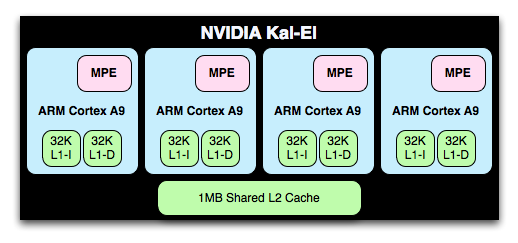
\includegraphics[width=0.9\textwidth]{figures/kalelcpu.png}
\end{center} \end{figure}

\end{frame}

% \begin{frame} 
% \frametitle{ARM A5}
% Combinatie A8 en een low power core
% \end{frame}

\begin{frame} 
\frametitle{ARM A15}

\begin{itemize}
 \item Nieuw design: high performance
 \item Zal de komende maanden worden ge\"introduceerd in tablet en smarthones.
\end{itemize}

\end{frame}



\begin{frame} 
\frametitle{ARM demo films}
  \begin{itemize}
  \item <1-> Beagle Board Description: \url{http://www.youtube.com/watch?v=fEL0sW71PFs}
  \item <2-> Beagle Board xM: \url{http://www.youtube.com/watch?v=9E31p3_eE28}
  \item <3-> ARM - 20 Years of partnership and innovation: \url{http://www.youtube.com/watch?v=JSmbS6GziS0}
  \item <4-> NVIDIA unveils Tegra 2: \url{http://www.youtube.com/watch?v=mlOTcs-effU}
  \item <5-> ARM Cortex-A15 MPcore processor: \url{http://www.youtube.com/watch?v=vF0ALmcCiLA}
  \end{itemize} 
\end{frame}

\end{document}
